\hypertarget{tsp_8c}{
\section{lib/tsp.c File Reference}
\label{tsp_8c}\index{lib/tsp.c@{lib/tsp.c}}
}
TSP solver and Lin-Kernighan heuristic. 

{\tt \#include \char`\"{}arrow.h\char`\"{}}\par


Include dependency graph for tsp.c:\nopagebreak
\begin{figure}[H]
\begin{center}
\leavevmode
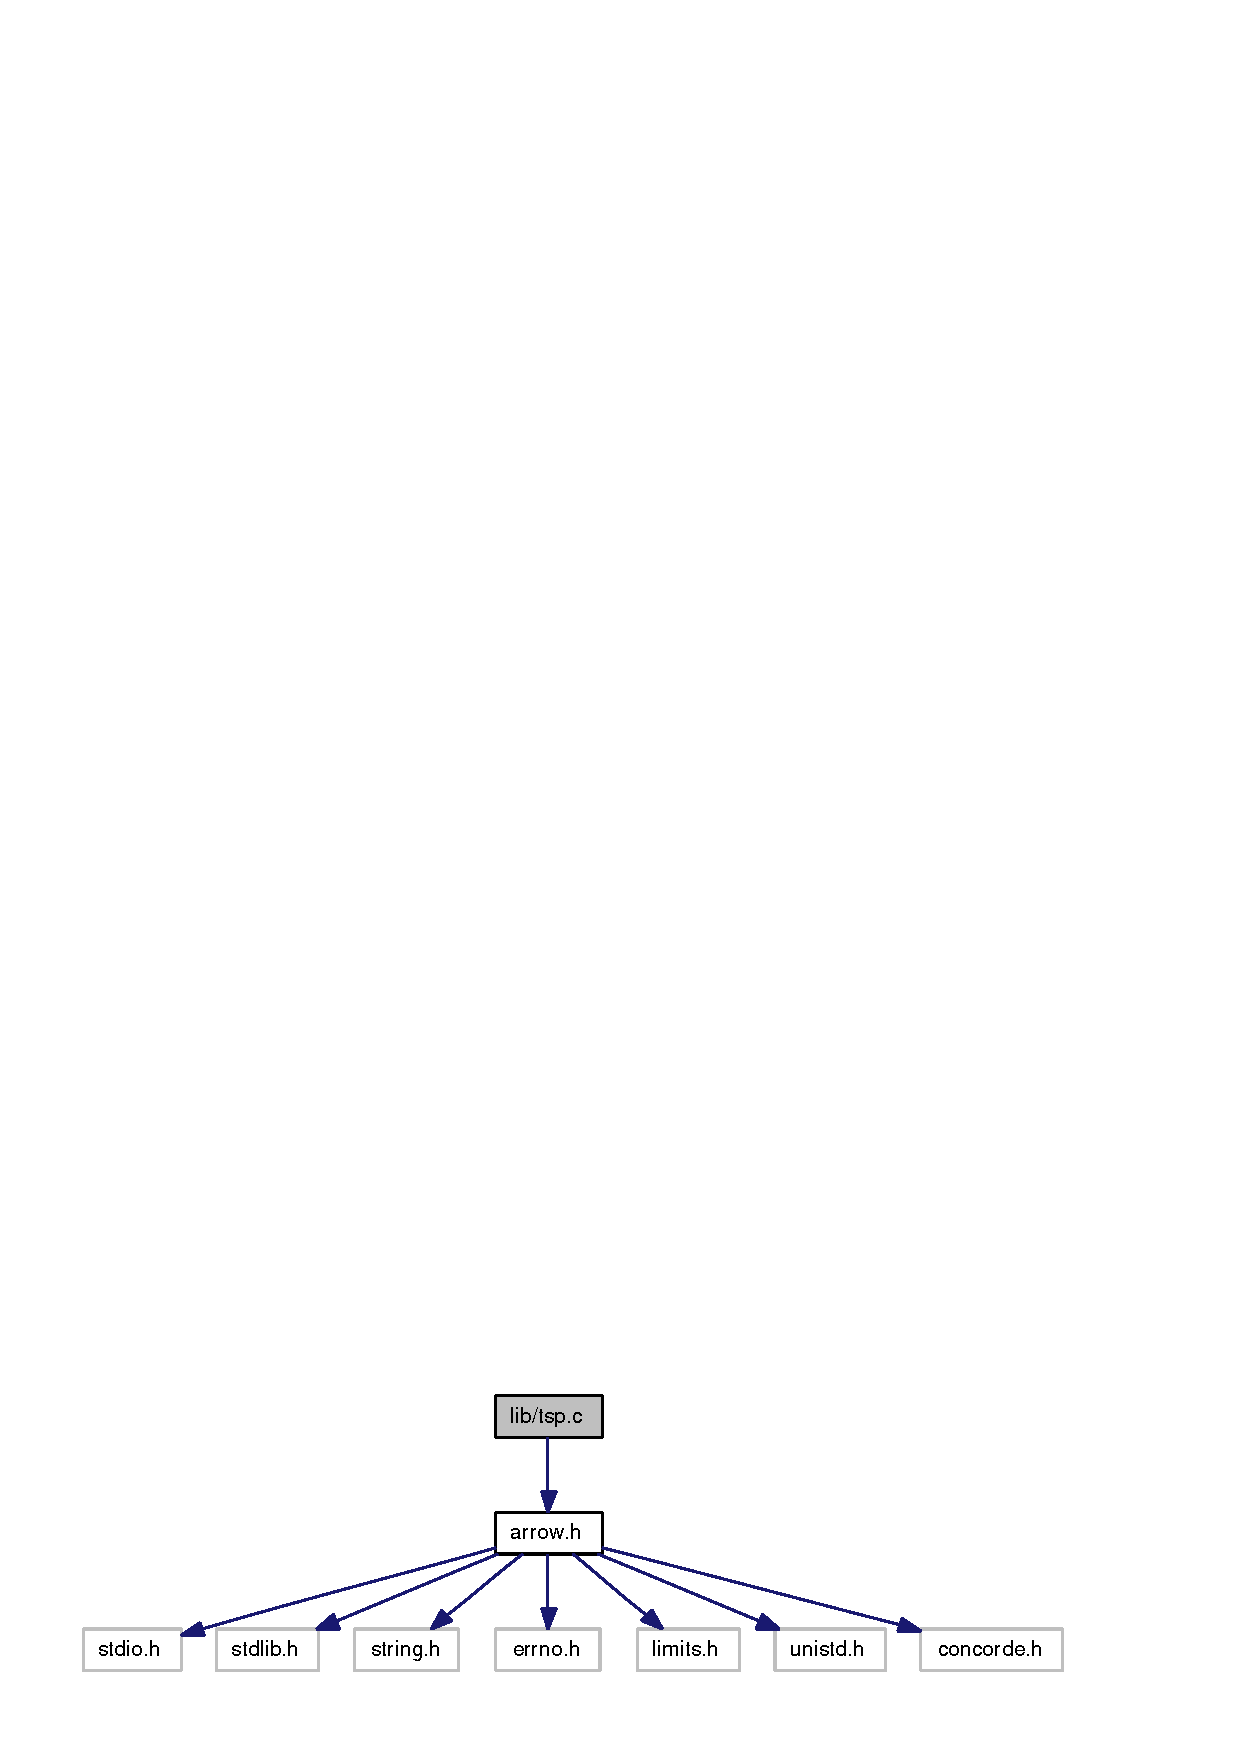
\includegraphics[width=257pt]{tsp_8c__incl}
\end{center}
\end{figure}
\subsection*{Functions}
\begin{CompactItemize}
\item 
void \hyperlink{tsp_8c_107b3fa0e8b3eeab9e04320d30654ec5}{arrow\_\-tsp\_\-result\_\-init} (\hyperlink{structarrow__problem}{arrow\_\-problem} $\ast$problem, \hyperlink{structarrow__tsp__result}{arrow\_\-tsp\_\-result} $\ast$result)
\begin{CompactList}\small\item\em Initializes the TSP result structure. \item\end{CompactList}\item 
void \hyperlink{tsp_8c_0665c82047dc78f8d08f12ecf5a9eef8}{arrow\_\-tsp\_\-result\_\-destruct} (\hyperlink{structarrow__tsp__result}{arrow\_\-tsp\_\-result} $\ast$result)
\begin{CompactList}\small\item\em Destructs a TSP result structure. \item\end{CompactList}\item 
void \hyperlink{tsp_8c_a20fdb653581bbcfcd08784900b19218}{arrow\_\-tsp\_\-lk\_\-params\_\-default} (\hyperlink{structarrow__problem}{arrow\_\-problem} $\ast$problem, \hyperlink{structarrow__tsp__lk__params}{arrow\_\-tsp\_\-lk\_\-params} $\ast$params)
\begin{CompactList}\small\item\em Sets default parameters for Lin-Kernighan heuristic:\begin{itemize}
\item stall\_\-count = problem-$>$size\item kicks = 0\item kick\_\-type = CC\_\-LK\_\-GEOMETRIC\_\-KICK\item time\_\-bound = 0.0\item length\_\-bound = 0.0\item initial\_\-tour = NULL. \end{itemize}
\item\end{CompactList}\item 
int \hyperlink{tsp_8c_0cc68200bf38d20fe0dd3c388674d215}{arrow\_\-tsp\_\-exact\_\-solve} (\hyperlink{structarrow__problem}{arrow\_\-problem} $\ast$problem, int $\ast$in\_\-tour, \hyperlink{structarrow__tsp__result}{arrow\_\-tsp\_\-result} $\ast$result)
\begin{CompactList}\small\item\em Solves TSP with Concorde's exact solver. \item\end{CompactList}\end{CompactItemize}


\subsection{Detailed Description}
TSP solver and Lin-Kernighan heuristic. 

Wrapper for calling Concorde's TSP solver and Lin-Kernighan heuristic.

\begin{Desc}
\item[Author:]John LaRusic \end{Desc}


Definition in file \hyperlink{tsp_8c-source}{tsp.c}.

\subsection{Function Documentation}
\hypertarget{tsp_8c_0cc68200bf38d20fe0dd3c388674d215}{
\index{tsp.c@{tsp.c}!arrow\_\-tsp\_\-exact\_\-solve@{arrow\_\-tsp\_\-exact\_\-solve}}
\index{arrow\_\-tsp\_\-exact\_\-solve@{arrow\_\-tsp\_\-exact\_\-solve}!tsp.c@{tsp.c}}
\subsubsection{\setlength{\rightskip}{0pt plus 5cm}int arrow\_\-tsp\_\-exact\_\-solve ({\bf arrow\_\-problem} $\ast$ {\em problem}, \/  int $\ast$ {\em in\_\-tour}, \/  {\bf arrow\_\-tsp\_\-result} $\ast$ {\em result})}}
\label{tsp_8c_0cc68200bf38d20fe0dd3c388674d215}


Solves TSP with Concorde's exact solver. 

\begin{Desc}
\item[Parameters:]
\begin{description}
\item[{\em problem}]\mbox{[}in\mbox{]} problem to solve \item[{\em in\_\-tour}]\mbox{[}in\mbox{]} an initial tour (can be NULL) \item[{\em result}]\mbox{[}out\mbox{]} TSP solution \end{description}
\end{Desc}


Definition at line 36 of file tsp.c.

References ARROW\_\-ERROR\_\-FATAL, ARROW\_\-ERROR\_\-NON\_\-FATAL, ARROW\_\-SUCCESS, arrow\_\-util\_\-zeit(), arrow\_\-problem::data, arrow\_\-tsp\_\-result::found\_\-tour, arrow\_\-problem::name, arrow\_\-problem::size, arrow\_\-tsp\_\-result::total\_\-time, arrow\_\-tsp\_\-result::tour, and arrow\_\-tsp\_\-result::tour\_\-length.\hypertarget{tsp_8c_a20fdb653581bbcfcd08784900b19218}{
\index{tsp.c@{tsp.c}!arrow\_\-tsp\_\-lk\_\-params\_\-default@{arrow\_\-tsp\_\-lk\_\-params\_\-default}}
\index{arrow\_\-tsp\_\-lk\_\-params\_\-default@{arrow\_\-tsp\_\-lk\_\-params\_\-default}!tsp.c@{tsp.c}}
\subsubsection{\setlength{\rightskip}{0pt plus 5cm}void arrow\_\-tsp\_\-lk\_\-params\_\-default ({\bf arrow\_\-problem} $\ast$ {\em problem}, \/  {\bf arrow\_\-tsp\_\-lk\_\-params} $\ast$ {\em params})}}
\label{tsp_8c_a20fdb653581bbcfcd08784900b19218}


Sets default parameters for Lin-Kernighan heuristic:\begin{itemize}
\item stall\_\-count = problem-$>$size\item kicks = 0\item kick\_\-type = CC\_\-LK\_\-GEOMETRIC\_\-KICK\item time\_\-bound = 0.0\item length\_\-bound = 0.0\item initial\_\-tour = NULL. \end{itemize}


\begin{Desc}
\item[Parameters:]
\begin{description}
\item[{\em problem}]\mbox{[}in\mbox{]} problem to solve \item[{\em params}]\mbox{[}out\mbox{]} LK parameters structure \end{description}
\end{Desc}


Definition at line 29 of file tsp.c.\hypertarget{tsp_8c_0665c82047dc78f8d08f12ecf5a9eef8}{
\index{tsp.c@{tsp.c}!arrow\_\-tsp\_\-result\_\-destruct@{arrow\_\-tsp\_\-result\_\-destruct}}
\index{arrow\_\-tsp\_\-result\_\-destruct@{arrow\_\-tsp\_\-result\_\-destruct}!tsp.c@{tsp.c}}
\subsubsection{\setlength{\rightskip}{0pt plus 5cm}void arrow\_\-tsp\_\-result\_\-destruct ({\bf arrow\_\-tsp\_\-result} $\ast$ {\em result})}}
\label{tsp_8c_0665c82047dc78f8d08f12ecf5a9eef8}


Destructs a TSP result structure. 

\begin{Desc}
\item[Parameters:]
\begin{description}
\item[{\em result}]\mbox{[}out\mbox{]} TSP result structure \end{description}
\end{Desc}


Definition at line 22 of file tsp.c.

References arrow\_\-tsp\_\-result::tour.\hypertarget{tsp_8c_107b3fa0e8b3eeab9e04320d30654ec5}{
\index{tsp.c@{tsp.c}!arrow\_\-tsp\_\-result\_\-init@{arrow\_\-tsp\_\-result\_\-init}}
\index{arrow\_\-tsp\_\-result\_\-init@{arrow\_\-tsp\_\-result\_\-init}!tsp.c@{tsp.c}}
\subsubsection{\setlength{\rightskip}{0pt plus 5cm}void arrow\_\-tsp\_\-result\_\-init ({\bf arrow\_\-problem} $\ast$ {\em problem}, \/  {\bf arrow\_\-tsp\_\-result} $\ast$ {\em result})}}
\label{tsp_8c_107b3fa0e8b3eeab9e04320d30654ec5}


Initializes the TSP result structure. 

\begin{Desc}
\item[Parameters:]
\begin{description}
\item[{\em problem}]\mbox{[}in\mbox{]} problem to solve \item[{\em result}]\mbox{[}out\mbox{]} TSP result structure \end{description}
\end{Desc}


Definition at line 12 of file tsp.c.

References ARROW\_\-FALSE, arrow\_\-util\_\-create\_\-int\_\-array(), arrow\_\-tsp\_\-result::found\_\-tour, arrow\_\-problem::size, arrow\_\-tsp\_\-result::total\_\-time, arrow\_\-tsp\_\-result::tour, and arrow\_\-tsp\_\-result::tour\_\-length.